\clearpage
\section{Homogenous Coordinates} \label{sec:homogenous}

The standard Cartesian coordinate system has long served as the foundation for representing points and vectors in Euclidean space. However, certain limitations arise when dealing with transformations, particularly translations and perspective projections, both of which are operations core to this paper. To overcome these challenges, homogenous coordinates are employed.

\begin{definition}
    Given a point $(a_1, a_2, \cdots, a_n) \in \Real^n$, it can be expressed in homogenous coordinates as $(\lambda a_1, \lambda a_2, \cdots, \lambda a_n, \lambda) \in \Real^{n+1}$, where $\lambda \neq 0$ is a constant scale factor. 
\end{definition}

In other words, we essentially extend the coordinate representation to include an extra dimension

\begin{equation}
    \begin{bmatrix}
        u \\ v 
    \end{bmatrix}
    \sim
    \begin{bmatrix}
        u\widetilde{w} \\ v\widetilde{w} \\ \widetilde{w}
    \end{bmatrix}
    \equiv
    \begin{bmatrix}
        \widetilde{u} \\ \widetilde{v} \\ \widetilde{w}
    \end{bmatrix}
\end{equation}

One important property of homogenous coordinates is that if the homogenous coordinate of a point is multiplied by a non-zero scalar, the result represents the same point. i.e.
\begin{equation}
    \begin{bmatrix}
        \widetilde{u} \\ \widetilde{v} \\ \widetilde{w}
    \end{bmatrix}
    \equiv
    k
    \begin{bmatrix}
        \widetilde{u} \\ \widetilde{v} \\ \widetilde{w}
    \end{bmatrix}
    \qquad (k \neq 0)
\end{equation}

\begin{figure}[H]
    \centering
    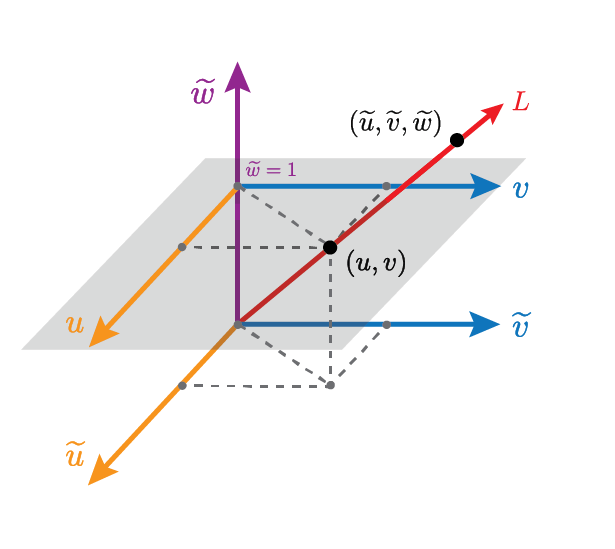
\includegraphics[width=0.6\textwidth]{diagrams/homogenous}
    \caption{Homogenous coordinate system.}
\end{figure}
